% =====================================================================
%  FraudLens - Slide A flow : Building the Data Foundation (blocks 1-5)
%  Compile:  pdflatex flow_a.tex
%  PNG    :  pdftoppm -r 400 -png flow_a.pdf flow_a
% =====================================================================
\documentclass[border=5pt]{standalone}

\usepackage[T1]{fontenc}
\usepackage{tikz}
\usetikzlibrary{arrows.meta}
\hyphenpenalty=10000 \exhyphenpenalty=10000

\definecolor{hiFill}{HTML}{E6E6F7}
\definecolor{hiLine}{HTML}{2A2A8C}
\definecolor{inkCol}{HTML}{111111}

\begin{document}
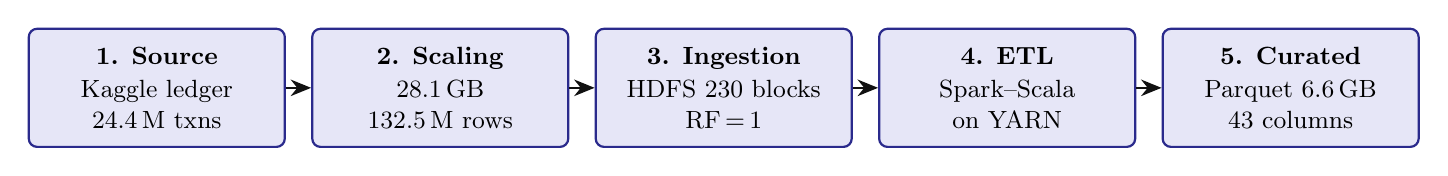
\begin{tikzpicture}[
  font=\small,
  blk/.style={
    draw=hiLine, line width=0.8pt, rounded corners=3pt,
    fill=hiFill, align=center, inner sep=5pt,
    text width=29mm, minimum height=15mm
  },
  ar/.style={-{Stealth[length=2.6mm,width=2.1mm]}, line width=0.8pt, inkCol}
]

\def\cx{36mm}

\node[blk] (a1) at (0*\cx,0) {\textbf{1. Source}\\[1pt]Kaggle ledger\\24.4\,M txns};
\node[blk] (a2) at (1*\cx,0) {\textbf{2. Scaling}\\[1pt]28.1\,GB\\132.5\,M rows};
\node[blk] (a3) at (2*\cx,0) {\textbf{3. Ingestion}\\[1pt]HDFS 230 blocks\\RF\,=\,1};
\node[blk] (a4) at (3*\cx,0) {\textbf{4. ETL}\\[1pt]Spark--Scala\\on YARN};
\node[blk] (a5) at (4*\cx,0) {\textbf{5. Curated}\\[1pt]Parquet 6.6\,GB\\43 columns};

\draw[ar] (a1) -- (a2);
\draw[ar] (a2) -- (a3);
\draw[ar] (a3) -- (a4);
\draw[ar] (a4) -- (a5);

\end{tikzpicture}
\end{document}
